\documentclass{article}
\usepackage{amsmath}
\usepackage{amssymb}
\usepackage{graphicx}
\usepackage{hyperref}
\usepackage[version=4]{mhchem}


\begin{document}
\(A B C D\) is a parallelogram. \(D E \perp A B\) at \(E . A D=\frac{1}{2} F C\). Show that \(\angle D A B=3 \angle A C D\).

Solution:
\begin{center}
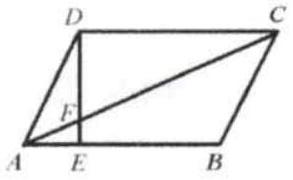
\includegraphics[width=\textwidth]{images/012(1).jpg}
\end{center}

Draw \(D N\), the median of triangle \(C D F\). Since \(D N\) is the median, by Theorem 1.3, \(D N=F N=N C\).\\
Since \(A D=\frac{1}{2} F C, A D=D N\).\\
Thus triangle \(A N D\) is an isosceles triangle with \(\angle D A N=\angle D N A\).\\
\centering
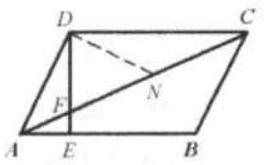
\includegraphics[width=\textwidth]{images/012(2).jpg}

We also know that \(D N=N C\), so \(\angle N D C=\angle N C D\).\\
\(\angle D N A\) is the exterior angle of triangle \(D N C\). So \(\angle D N A=\angle N D C+\angle N C D\)\\
\(=2 \angle N C D\).\\
Note that \(\angle C A B=\angle N C D\).\\
Therefore \(\angle D A B=\angle D C A+\angle C A B=\angle D N A+\angle N C D\)\\
\(=2 \angle N C D+\angle N C D=3 \angle N C D=3 \angle A C D\).


\end{document}
